% This is the actual main file of the REPORT (thesis) being written. It calls upon
% other files like the header, footer, as well as each of the individual chapters.
% The structure is pretty straightforward. 
% 
% The location of each of the files: 
% - docsettings/header.tex: contains all the document info, the pakages used and 
% macros defined.
% - docsettings/titlepage.tex: Contains the title page of the document, in case a 
% specific one is required.
% - docsettings/prologue.tex: Contains statements, acknowledgements, etc...
% that would go before the actual contents.
% - chapters/intro.tex: Introductory chapter.
% - chapters/chaptX.tex: Chapter X in the document.
% - chapters/conclusion.tex: Final chapter.
% - chapters/appY.tex: Appendix number Y of the document.
%
% It is advisable to place all the images within the ./pics folder, 
% which is already preselected to hold the images. 
%
% 
\documentclass[fontsize=9.5pt,
    a4paper,
    oneside, % twoside also available
    index=totoc,
    parskip=half,
    chapterprefix]{scrbook}
% In case you're using an earlier version of LaTeX
\usepackage{etex}
\reserveinserts{28}

% Use utf-8 encoding for foreign characters
\usepackage[utf8]{inputenc}  
%\usepackage[LGR,T1]{fontenc}    

% If Spanish characters are required.
\usepackage[greek,spanish]{babel}  
\usepackage[pdftex]{graphicx}

% Setup for fullpage use and change geometry:
\usepackage[paperwidth=170mm, paperheight=225mm, margin=20mm]{geometry}
%\usepackage{geometry}
\usepackage{fullpage}

%Setup for multicolumn use
\usepackage{multicol}
\usepackage{multirow}
\usepackage{amsmath}
\usepackage{amssymb}
\usepackage{float}
\usepackage{textcomp}
\usepackage{tikz}
\usepackage{IEEEtrantools}
\usepackage{circuitikz}
\usepackage{pgfplots}
\usepackage{verbatim}
\usepackage{schemabloc}
\usepackage{latexsym}
\usepackage{lscape}
\usepackage{subfigure}
\usepackage{listofsymbols}
%\usepackage[final]{listofsymbols} Use only for the final run TeX run.
\usepackage{yfonts}
\usepackage{mathabx}

%\usepackage[pdf]{pstricks}

\usepackage{longtable}
\usepackage{tabularx}
%\usepackage{graphics}
\usepackage{listings}
\usepackage{array}
\usepackage[refpages]{gloss}
\usepackage{textgreek}
\usepackage[numbers]{natbib} % you're welcome on your awesome bibliography

\definecolor{LinkColor}{rgb}{0,0,0}
\usepackage[%
    pdftitle={PDF Title},%
    pdfauthor={Author},%
    pdfcreator={LaTeX with hyperref},
    pdfsubject={PDF Subject},
    pdfkeywords={keywords here}]{hyperref}
\hypersetup{colorlinks=true,%
    linkcolor=LinkColor,%
    citecolor=LinkColor,%
    filecolor=LinkColor,%
    menucolor=LinkColor,%
    pagecolor=LinkColor,%
    urlcolor=LinkColor}
  
\definecolor{lightblue}{rgb}{0.8,0.85,1}
\lstset{backgroundcolor=\color{lightblue}}

% easy MATLAB code input (you need to get mcode first)
%\usepackage[framed,numbered]{mcode}

\graphicspath{{./pics/}}

%----------------------------------
% Macros and definitions of the work.
%----------------------------------

% contiene código de MATLAB
% -----usage: \lstinputlisting{archivoMatlab.m}
% -----en lugar de : 
%           \lstinputlisting{/Users/JoseAlonso/Documents/MATLAB/archivoMatlab.m}
\newcommand{\autor}{José Alonso Solís Lemus}
\newcommand{\titulo}{TITLE OF THE DOCUMENT (THESIS or REPORT)}

% Caracteres extraños
\newcommand{\tildeps}{\tilde{\epsilon}}
\newcommand{\uu}{\mathbf{u}}
\DeclareMathOperator{\seno}{sen}
% teoremas y así
\newtheorem{teo}{Theorem}
\newtheorem{dfn}{Definition}
% ---------------------------------
\makegloss

%Si no se quieren hojas numeradas
%\pagestyle{headings}
%----------------------------------
\begin{document}
%\nocite{*}
%---------------------------------
\thispagestyle{empty}
\setcounter{page}{1}
\begin{center}\vspace{70pt}
\begin{tabular}{c}
\hline
\large \emph{\textsc{University or Institution name}}\\
\hline
\end{tabular}\\
\vspace{30pt}
\includegraphics[width=10cm,height=2.8cm]{Logo_ITAM.jpeg}\\
\vspace{30pt}
\Large \titulo \\
\vspace{30pt}
\normalsize {THESIS}\\
\vspace{10pt}
QUE PARA OBTENER EL TÍTULO DE\\
\vspace{5pt}
{\large Ingeniero en Telemática}\\
\vspace{35pt}
PRESENTA\\
\vspace{5pt}
{\large \autor } \\
\vspace{35pt}
SUPERVISOR: Dr. Someone Important\\
\vspace{22pt}
\begin{tabular}{lcr}
LOCATION & \hspace{85pt} & \today\year
\end{tabular}
\end{center}
%\newpage
%\setcounter{page}{1}
\pagenumbering{roman}
\mbox{ }
\vspace{85pt}
\mbox{ }
\newpage
\pagenumbering{roman}
%for 1.2 sptacing:
%\renewcommand{\baselinestretch}{1.20}\normalsize
%---------------------------------
%\addcontentsline{toc}{chapter}{Declaration}
\chapter*{Declaration}
The work here presented is mine, except where explicitly cited.


\newpage
%$%$%$  ------------------------------------------------------------------------------------  $%$%$%
%\chapter*{\phantom{Dedications}}
%\begin{flushright}
%\emph{
%For person number 1 who's really important. \bigskip\\
%Also for people number 2 cause he's cool... \bigskip\\
%}
%\end{flushright}
%$%$%$  ------------------------------------------------------------------------------------  $%$%$%
%\chapter*{Acknowledgements}
%\begin{flushright}
%\emph{Acknowledgement number 1. \bigskip\\
%Acknowledgement number 2 ...
%}
%\end{flushright}
%$%$%$  ------------------------------------------------------------------------------------  $%$%$%






\chapter*{Abstract}
Abstract of your document goes here...
\newpage
%---------------------------------
\tableofcontents
\listoffigures
\listoftables
\listofsymbols 
\opensymdef
\newsym[Variable en negritas equivale a un vector.]{symu}{\textbf{u}}
\newsym[Densidad de masa del fluido.]{symrho}{\rho}
\newsym[Derivada sustancial o material.]{symddt}{D\slash Dt}
\newsym[Número Mach de la onda, definido como el cociente de la velocidad pico de la onda con la velocidad del sonido. Utilizado para hacer aproximaciones.]{symmach}{\epsilon}
\newsym[N\'umero utilizado como referencia para aproximaciones.]{symeta}{\eta}
\newsym[Representación de fuerzas tensoras.]{symtensor}{\Upsilon}
\newsym[Densidad lagrangiana de segundo orden.]{symlagrangian}{\mathcal{L}}
\newsym[Operador de D'Alambert.]{symalambert}{\Box}
\newsym[Operador gradiente.]{nablauno}{\nabla}
\newsym[Operador Laplaciano definido por $\nabla^2 = \nabla\cdot\nabla$,normalmente denotado por $\bigtriangleup$.]{nablados}{\nabla^2}
\newsym[Operador Laplaciano en el plano ortogonal al eje de propagación.]{nabladosbot}{\nabla^2_{\bot}}
\newsym[Representación de orden.]{orden}{O(\cdot)}
\newsym[Velocidad pico de la se\~nal.]{ucero}{u_0}
\newsym[Velocidad constante del sonido.]{ccero}{c_0}
\newsym[Valores de viscosidad de cizallamiento y de volúmen.]{mumu}{\mu,\mu_B}
\newsym[Variables utilizadas para frecuencia angular y lineal.]{fomega}{\omega,f}
\newsym[Constante de no linelidad del medio.]{nolin}{\beta}
\newsym[Constante de conductividad térmica.]{conductterm}{\kappa}
\newsym[Constante de disipación del medio.]{disipacion}{\delta}
\newsym[Densidad del medio.]{rhocero}{\rho_0}
\newsym[Constante de atenuación (dependiente de $x$).]{alphax}{\alpha_x}
\newsym[Constante de referencia de temperatura.]{Tcero}{T_0}
\newsym[Complejo conjugado (c.c) de $x$.]{complejox}{\bar{x},\text{c.c}}
\newsym[Viscosidad cinemática $\nu = \mu\slash\rho$.]{visccine}{\nu}
\newsym[Constantes de coeficientes de calor espec\'ifico a presión y volúmen constante.]{cvcp}{c_p,c_v}
\newsym[Presión sonora inicial de la se\~nal.]{pcero}{p_0}
\newsym[Longitud de onda.]{longitudonda}{\lambda}
\newsym[Número de onda, definido como $2\pi\slash\lambda$.]{numeroonda}{k}
\newsym[Radio de la bocina direccional.]{radioa}{a}
\newsym[Distancia de Rayleigh.]{rayleigh}{R(k,a)}
\newsym[Función de Green para la onda $n$.]{greenfunc}{G_n(\cdot,\cdot)}
\newsym[Funciones de directividad de apertura y de Westervelt.]{dadw}{D_A,D_W}
\newsym[Función de Bessel del primer tipo de orden $n$.]{besseln}{J_n}
\newsym[Función de Heaviside.]{heaviside}{H(\cdot)}
\newsym[Función moduladora.]{envelope}{E(t)}
\newsym[Delta de Kronecker.]{deltakron}{\delta_{i,j}}
\newsym[Variables utilizadas para la presión sonora.]{Pp}{P,p}
\newsym[Variable utilizada para denotar la entrop\text{\'i}a.]{entropia}{s}
\newsym[Variable utilizada para la temperatura.]{temperatura}{T}
%\newsym[Norma bajo el espacio de Sobolev $H^S$.]{hsupers}{\Vert\cdot\Vert_{H^S}}
\closesymdef
\newpage
\pagenumbering{arabic}
%---------------------------------
\chapter{Introduction}
% If you don't want quotes, comment the next lines.
\begin{flushright}
Cool quote at the begining of first chapter...\\
\emph{- Someone awesome (Extract from...) -}
\end{flushright}
Some introduction on the topic to talk about. Maybe you're talking about nonlinear 
acoustics and directional speakers. Maybe talk on this chapter about the the concept,
be sure to define the problem and some of the pathway to solving it. Don't 
overcomplicate it. \medskip\\
This chapter should define the problems you want to address, the objectives, the 
scope, methodology and structure of the document.
\section{Definition of the problem} % Planteamiento del problema
El problema a resolver en este trabajo es modelar matemáticamente el comportamiento 
de una bocina direccional\footnote{everyone loves footnotes, so throw some in there!}
,...
\section{Objectives and Scope}
You must be able to determine a list of objectives you want to fulfill, and how far
does your research contemplate. Maybe something like:
\begin{itemize}
\item Build the math models, trying to make sense of them into your application. You 
want to understand further the phenomena you're studying, and math is a great tool.
\item Maybe some practical work might be in order, like a programing or an actual 
experiment
\item Throw in something exiting and new.
\end{itemize}
Since you can't cover absolutely everything, it is smart to talk about the scope of
your work. Where it fails, what won't it consider...
\section{Structure and methodology}
Methodology to solve the problem, and structure to explain what is going to be 
covered and where on the document. I sense another list coming...
\begin{figure}[hbpt]
\centering
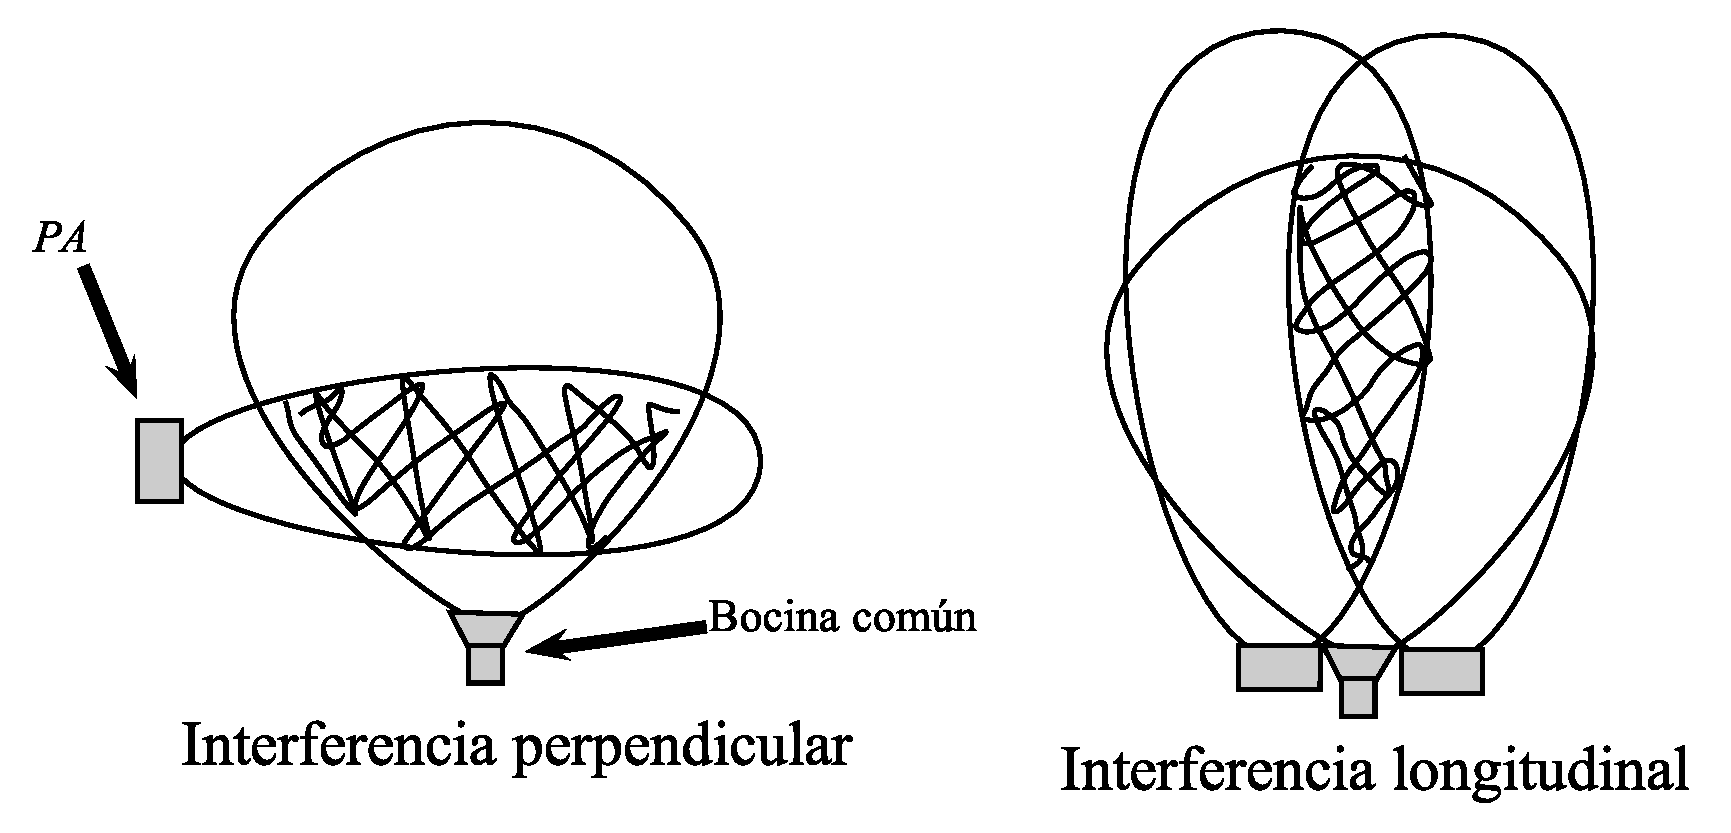
\includegraphics[scale=0.31]{introexp}
\caption{Caption for the image (Where did you get this?)}
\label{fig:introexp}
\end{figure}
Explain Figure \ref{fig:introexp} properly. 
%---------------------------------
%
% --------------------------------
\chapter{La ecuación de Khokhlov–Zabolotskaya–Kuznetsov}\label{chapter.kzk}
\begin{flushright}
Shock waves, bones to dust\\
You're messin' with a mine field\\
so expect the worst\\
\emph{- Judas Priest (Hard as Iron)-}
\end{flushright}

La ecuación Khokhlov–Zabolotskaya–Kuznetsov (KZK) fue derivada originalmente como una herramienta para la descripción de rayos acústicos no lineales dentro de un medio. Describe la propagación no lineal de un pulso de amplitud finita de un haz de sonido en un medio termo-viscoso. La ecuación, describe con exactitud el proceso entero de auto-demodulación de una señal ultrasónica, a lo largo del campo cercano y hacia el campo lejano. ...
\section{Derivación de la ecuación KZK} 
 Las fuentes de ultrasonido generan fenómenos muy marcados de difracción, que se combinan con los efectos de amplitud finita para producir formas de onda que varían de un punto a otro dentro del haz de sonido. El énfasis en esta sección es la derivación de la ecuación KZK. Se puede probar, en el artículo de Rozanova-Pierrat \cite{mathkzk}, que el problema de la ecuación KZK ...
\begin{figure}[hbpt]
\centering
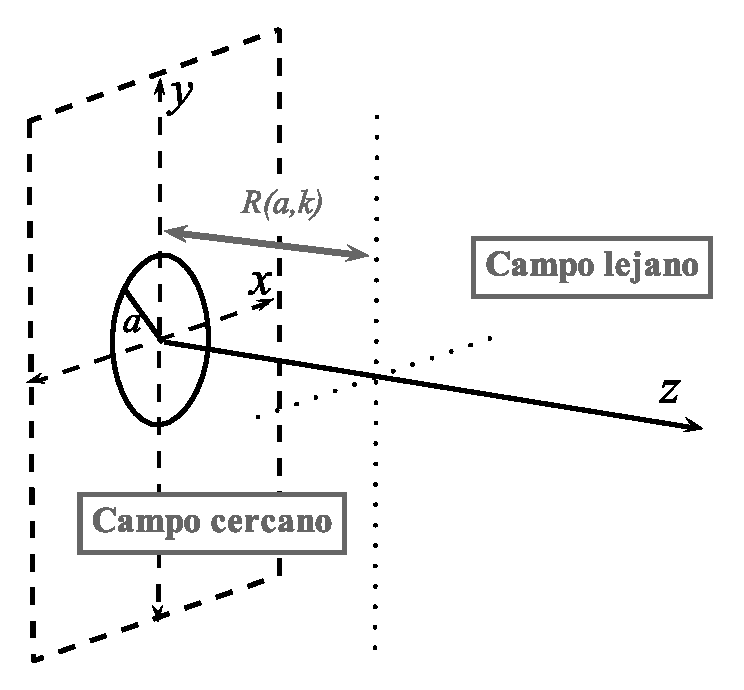
\includegraphics[scale=0.5]{ejepropagacion}
\caption{Esquema del eje de propagación y el radio de la fuente.}
\label{fig:propagacion}
\end{figure}
Normalmente, se caracteriza al campo sonoro de una forma muy similar a los campos electromagnéticos, ya que se clasifican con respecto a la cercanía a la fuente en campo cercano y lejano. Éste, empezando aproximadamente en la distancia de Rayleigh $R(a,k) = (ka^2)\slash2$, medida desde la...
\begin{align*}
& \tildeps\frac{1}{c_0^2}\frac{\partial^2p}{\partial \tau^2} +\tildeps\frac{\delta}{c_0^4}\frac{\partial^3p}{\partial \tau^3}  = -\tildeps^2\frac{\beta}{\rho_0c_0}\frac{\partial^2p^2}{\partial \tau^2}\text{,}
\end{align*}
entonces:
\begin{align*}
&\tildeps\left[ \tildeps\left(\frac{\partial^2}{\partial x_1^2} +\frac{\partial^2}{\partial y_1^2}\right) + \tildeps^2 \frac{\partial^2}{\partial z_1^2} - \tildeps\frac{2}{c_0} \frac{\partial^2}{\partial z_1\partial \tau} +\frac{1}{c_0^2}\frac{\partial^2}{\partial \tau^2}\right]p - = \\
&\quad=-\tildeps^2\frac{\beta}{\rho_0c_0}\frac{\partial^2p^2}{\partial \tau^2}-\tildeps\frac{1}{c_0^2}\frac{\partial^2p}{\partial \tau^2} - \tildeps\frac{\delta}{c_0^4}\frac{\partial^3p}{\partial \tau^3}\text{,}
\end{align*}
de donde se sigue que:
\begin{align*}
&\left[\tildeps^2\left( \frac{\partial^2}{\partial x_1^2}+\frac{\partial^2}{\partial y_1^2}\right) + \tildeps^3\frac{\partial^2}{\partial z_1^2} - \tildeps^2 \frac{2}{c_0}\frac{\partial^2}{\partial z_1\partial \tau} +\frac{1}{c_0^2}\frac{\partial^2}{\partial \tau^2}\right]p - = \\
&\quad = -\tildeps^2\frac{\beta}{\rho_0 c_0}\frac{\partial^2p^2}{\partial \tau^2} - \tildeps\frac{1}{c_0^2}\frac{\partial^2p}{\partial \tau^2} -\tildeps\frac{\delta}{c_0^4}\frac{\partial^3p}{\partial \tau^3}\text{.}
\end{align*}
%
Únicamente es necesario eliminar de los cálculos el término de orden $O(\tildeps^3)$ para quedar con la ecuación siguiente:
%
\begin{align}
\tildeps\left( \frac{\partial^2}{\partial x_1^2} +\frac{\partial^2}{\partial y_1^2}\right)p +\frac{1}{c_0^2}\frac{\partial^2p}{\partial \tau^2} - \frac{1}{c_0^2}\frac{\partial^2p}{\partial \tau^2} - \tildeps \frac{2}{c_0}\frac{\partial^2p}{\partial z_1\partial \tau}+ \frac{\delta}{c_0^4}\frac{\partial^3p}{\partial \tau^3} = -\frac{\beta}{\rho_0 c_0}\frac{\partial^2p^2}{\partial \tau^2}\text{,}\nonumber \\
-\frac{c_0}{2}\times\left[\tildeps\left( \frac{\partial^2}{\partial x_1^2} +\frac{\partial^2}{\partial y_1^2}\right)p - \tildeps \frac{2}{c_0} \frac{\partial^2p}{\partial z_1\partial \tau}+
\frac{\delta}{c_0^4}\frac{\partial^3p}{\partial \tau^3}\right]  = -\frac{c_0}{2}\times\left[-\frac{\beta}{\rho_0 c_0}\frac{\partial^2p^2}{\partial \tau^2}\right] \label{eqn:prekzk}\text{.}
\end{align}
%
...

por lo que sí sería útil el desarrollo de un algoritmo que la pueda resolver apropiadamente.


%---------------------------------
%
%---------------------------------
%
%---------------------------------
\chapter{Conclusiones}
\begin{flushright} 
I was sick - sick unto death with that long agony...\\
\emph{- The Pit and the Pendulum-}\\
\emph{Edgar Allan Poe}
\end{flushright}


%---------------------------------
\newpage

% To make a glossary (not actually sure how...)
%\gloss[nocite]{*} \printgloss{glossary}

% command to update:: 
% makeindex -s baa_main.ist -t baa_main.glg -o baa_main.gls baa_main.glo

\newpage

% If you need it to say anything other than "Appendix"
%\addcontentsline{toc}{chapter}{Appendix}
%\appendix
%\input{chapters/appendix1}
%\input{chapters/appendix2}

\newpage
% If you need it to say anything that is not "References"
%\addcontentsline{toc}{chapter}{Bibliografía}

%%Added comment for this as it doesn't work right now

\bibliographystyle{unsrt} % or alpha, siam, IEEEtranN...
\bibliography{\myrefs} 
% you actually need a .bib file for this(Not included)
%
%
% YOU WILL NEED TO ADD THE BIB FILE HERE WITH YOUR REFERENCES.
% wE'LL DO THIS TOWARDS THE END WHEN YOU ACTUALLY HAVE A REPORT!!!
%
%
%
% \input{ZaiMPhil.bib} % We provided this, but it shouldn't be done this peasant way! 
